
\chapter{Introduction}

\outline{
    The first chapter should introduce the problem studied and describe the main results obtained in the thesis.
    In order to provide guidance to the reader, the first chapter should briefly describe the organization of the rest of the thesis.
    The first chapter can also give the background of previous work on the subject and the method used in attacking the problem.
}

With the end of Dennard scaling, computer architects have sough to satisfy demand for increasing performance by providing specialized hardware accelerators tuned to computation with particular characteristics.
Perhaps the most successful examples of this trend is the uniform adoption and IEEE 754 specification of floating-point hardware, and widespread adoption of graphics processing units (GPUs) for more general data-parallel compute tasks.
With the success of GPUs as a template, architects are moving forward with a wide variety of specialized processors, such as
SIMD extensions~\todo{cite NEON, SSE, AVX},
AI accelerators~\todo{google tpu, huawei neural processing unit, ibm neuromorphic},
motion coprocessors~\todo{cite apple},
field-programmable gate arrays (FPGAs)~\todo{cite Intel, Xilinx}
network processors~\todo{cite intel ixp, netronome},
digital signal processors~\todo{cite google pixel2},
vision processing units~\todo{cite movidius, microsoft, mobilieye, MIT},
and many others.

The degree to which these accelerators are integrated with the system varies.
Floating-point accelerators are fully integrated: they are part of the core instruction-set architecture, have first-class access to system memory, and are supported without specialized toolchains or programming systems.
GPUs vary from partially-integrated to discrete: when a GPU is integrated on the same die as the CPU, it may share the same physical memory, but the computation model remains for compute tasks to be ``offloaded'' to the GPU, with the CPU managing the execution.
Many GPUs, and the rest of the accelerators, are entirely discrete.
The interface with the CPU through a specialized vendor API, require separate toolchains and programming systems for compilation, and require explicit programmer effort to use their capabilities.

\begin{figure}[ht]
    \centering
    \includegraphics[width=0.5\textwidth,draft]{figures/integration-spectrum.png}
    \caption{Spectrum of system integration of accelerators. FLoating-point on the left, simd middle-left, some DSPs center, GPUs center to right, everything else on the right.}
    \label{fig:integration-spectrum}
\end{figure}

\begin{figure}
    \centering
    \begin{tikzpicture}[
        nodestyle/.style={},
        linestyle/.style={
            <->,
            very thick,
            shorten <=2pt,
            shorten >=2pt,}
        ]
        %Nodes
        \node[nodestyle] (n0) {Integrated};
        \node[nodestyle] (n1) [right=of n0] {Discrete}
         edge[linestyle] (n0.east);

        %Lines
        % \path (n0.east) edge [linestyle] node [above] {}    (n1.west);

    \end{tikzpicture}
    \caption{NVIDIA DGX-1 simple topology.}
    \label{fig:topo-dgx-simple}
\end{figure}

\begin{figure}
    \centering
    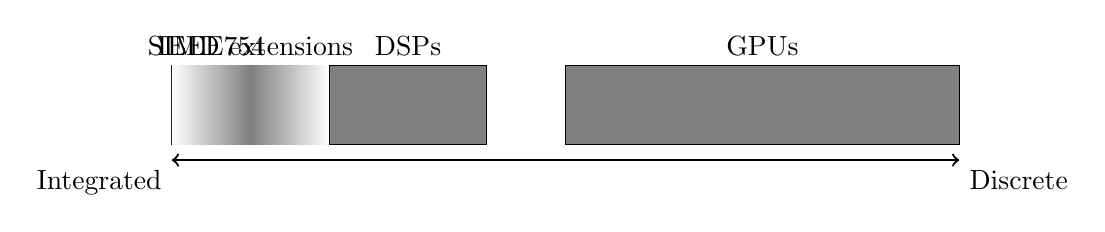
\begin{tikzpicture}[
        nodestyle/.style={},
        linestyle/.style={
            <->,
            very thick,
            shorten <=2pt,
            shorten >=2pt,}
        ]

        \draw[thick,<->] (0,0) node[anchor=north east] {Integrated} -- (10,0) node[anchor=north west] {Discrete};

        \draw[fill=gray] (0,0.2) rectangle (1,1.2);
        \node [above] at (0.5, 1.2) {IEEE \newline 754};

        \shade[left color=white, right color=gray] (0,0.2) rectangle (1,1.2);
        \shade[left color=gray, right color=white] (1,0.2) rectangle (2,1.2);
        \node [above] at (1, 1.2) {SIMD extensions};

        \draw[fill=gray] (2,0.2) rectangle (4,1.2);
        \node [above] at (3, 1.2) {DSPs};

        \draw[fill=gray] (5,0.2) rectangle (10,1.2);
        \node [above] at (7.5, 1.2) {GPUs};


    \end{tikzpicture}
    \caption{NVIDIA DGX-1 simple topology.}
    \label{fig:topo-dgx-simple}
\end{figure}

\outline{effort of management}

\outline{big data as a motivation, importance of communication}

\outline{work addresses both}

The rest of this document is organized as follows:
chapter 2 describes background and related work;
chapter 3 describes the hardware system characterization approach;
chapter 4 describes the application characterization approach;
chapter 5 describes the methodology for combining the system and application characterization to understand application performance;
chapter 6 discusses related work;
and finally, chapter 7 concludes.
